%TODO: obviously rewrite this
In this section I will describe the stack used for this thesis and the experiments done to achieve our results: I will start by reviewing the configurations and libraries utilized (par. \ref{bb}), the database used to acquire training and test set (par. \ref{rldb}), all the analysis done on the data (par. \ref{data_an}), and finally we will discuss the results of this work (par. \ref{results}).

\section{Building Blocks} \label{bb}
%TODO: maybe expand this with something?
To realize this work we used the following tools and libraries:
\begin{itemize}
	\item OpenFace: the library to train the models for face detection, landmark detection, feature extraction and action unit recognition.
	\item R + R-Studio: the environment where I implemented the code, with some important libraries, such as:
	\begin{itemize}
		\item e1071: library for SVM classification (implementation of libsvm).
		\item Random Forest: library to perform Random Forest and calculate variable importance.
		\item Corrplot: library for calculating and visualizing correlations.
	\end{itemize}
\end{itemize}

The experiments were conducted on two systems, Windows and Mac OS, with the following specs:\\
The windows machine has 8GB of RAM, i5 processor, and 4096MB ATI AMD Radeon R9. \\
The Mac has 4gb RAM, i5 processor, and an intel integrated GPU.\\
SVM training took about one hour on both machines.

\clearpage

%TODO: SHORT review (table pherhaps) of face db, maybe not in this section
\section{Real Life Trial Database} \label{rldb}
This section is about the database we used to perform our experiments: it comes from the work done for the paper "Deception Detection using Real-life Trial Data" \cite{Perez-Rosas:2015:DDU:2818346.2820758}.

\begin{figure}[H]
	\centering
	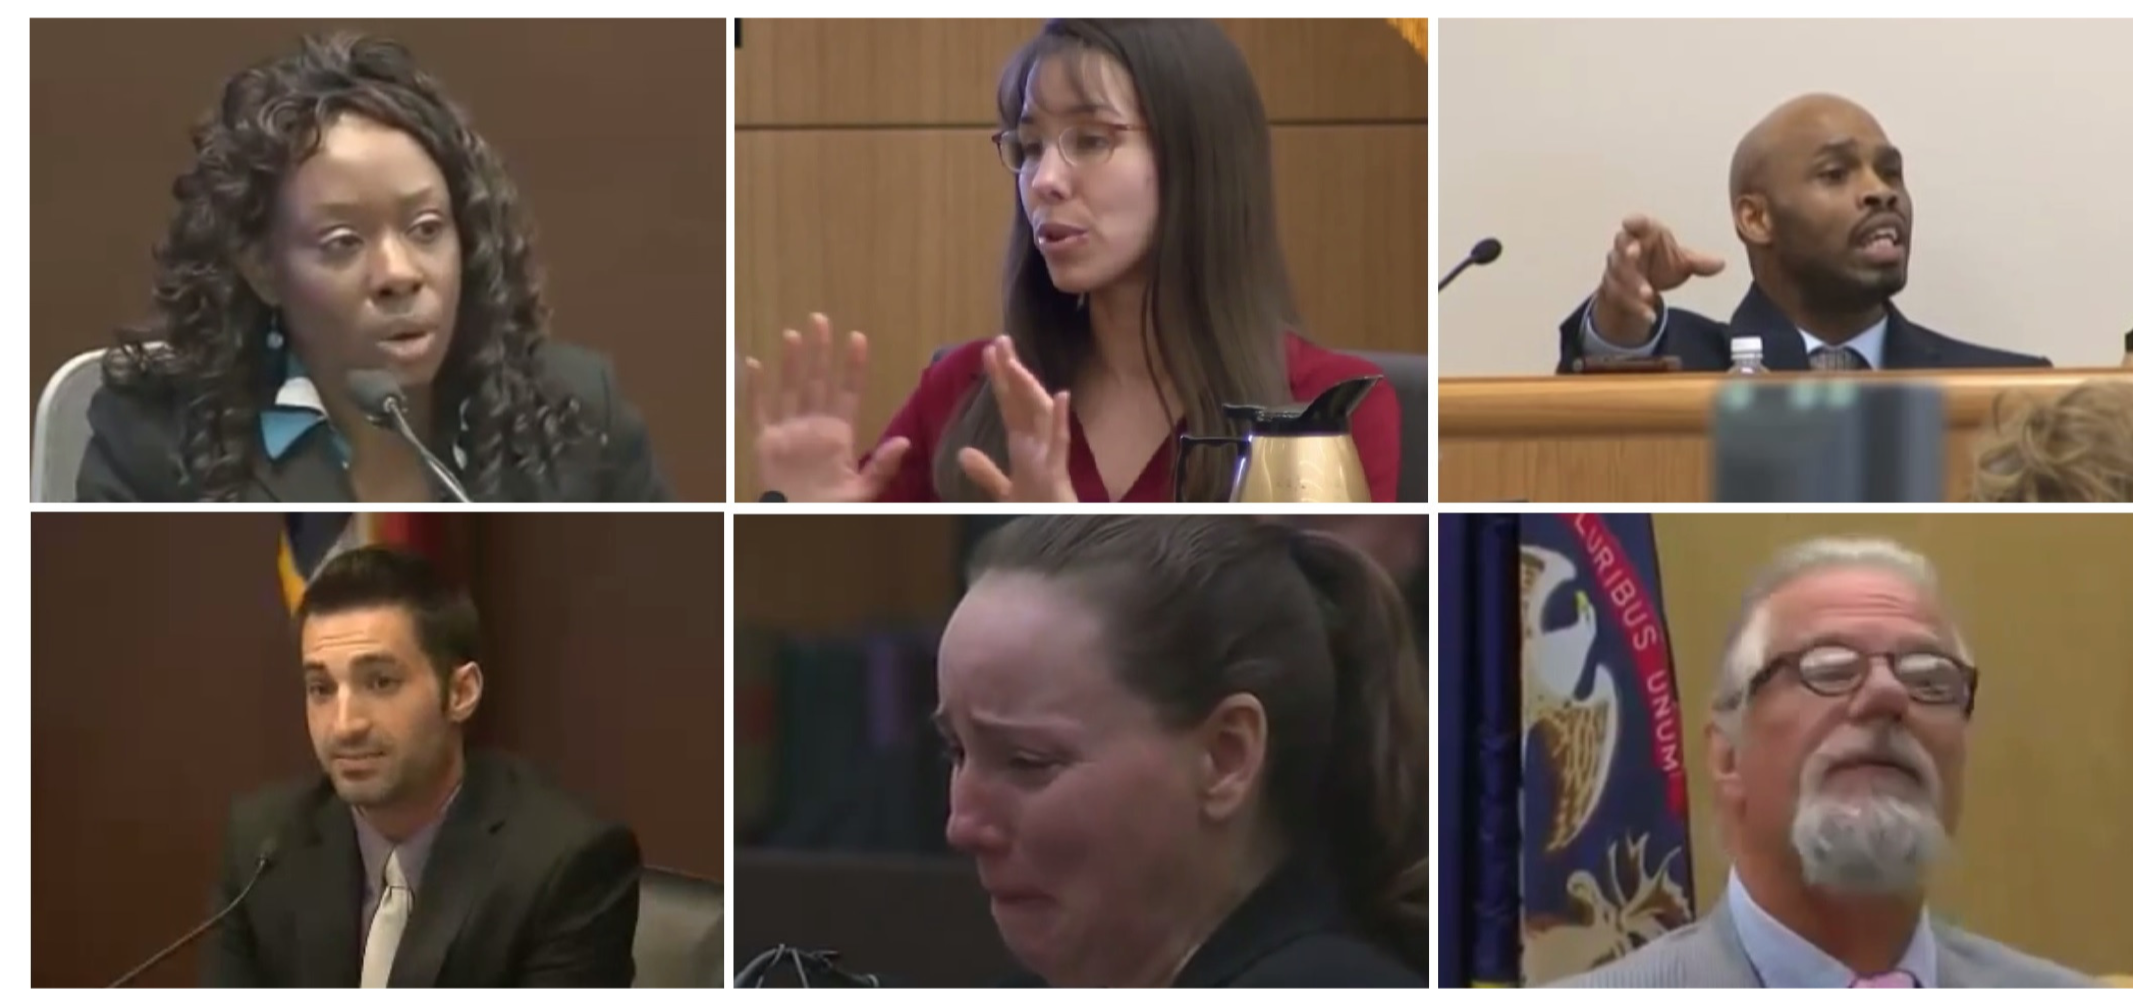
\includegraphics[width=1\textwidth]{trial_images}
	\caption{Examples of images from the dataset videos. \cite{Perez-Rosas:2015:DDU:2818346.2820758}.}
	\label{fig:trial_images}
\end{figure}


The dataset is gathered from real-life trial videos available on YouTube and other public websites. The dataset also contains statements made by exonerees after exoneration, and some statements from defendants during crime-related TV episodes.

The first step to collecting the dataset was to identify public multimedia sources where the recordings of the trials were available, and deceptive and truthful behavior could be observed and verified.\\
The videos are of trial recordings where the defendant or witness in the video can be clearly identified, the face is visible enough during most of the clip duration, and the visual quality should be good enough to accurately see the facial expressions (Fig. \ref{fig:trial_images}).\\
There are three outcomes for the trials that were considered to label the videos as deceptive or truthful: guilty, non-guilty, and exoneration. \\
For the guilty verdicts the deceptive clips are taken from the defendant in the trial, while the truthful clips are gathered from the witnesses. There are also instances where the deceptive videos are of suspects denying a committed crime, and truthful ones are from the same person answering questions that where verified by the police as truthful.

In regards to the witnesses, if the testimony is verified by a police officer they are labeled as true. \\ 
Testimonies that help the guilty party are labeled as false. Exoneration (reversal of the sentence) testimonies are regarded as truthful.

The original dataset consists of 121 videos, 61 of which are deceptive and 60 truthful. \\
The average length of the videos is 28.0 seconds. The average video length for deceptive videos is 27.7 seconds, while the one for truthful videos is 28.3 seconds. \\
The data consists of 58 total subject, 22 females and 36 males, with ages between 16 and 60 years.

This dataset was annotated following the MUMIN coding scheme for hand movement and facial displays. While annotating, the annotators were able to chose only one label per gesture, for every clip.

Fig. \ref{fig:rldb_distrib} shows the frequency counts associated with the gestures considered during the annotation.

\begin{figure}[H]
	\centering
	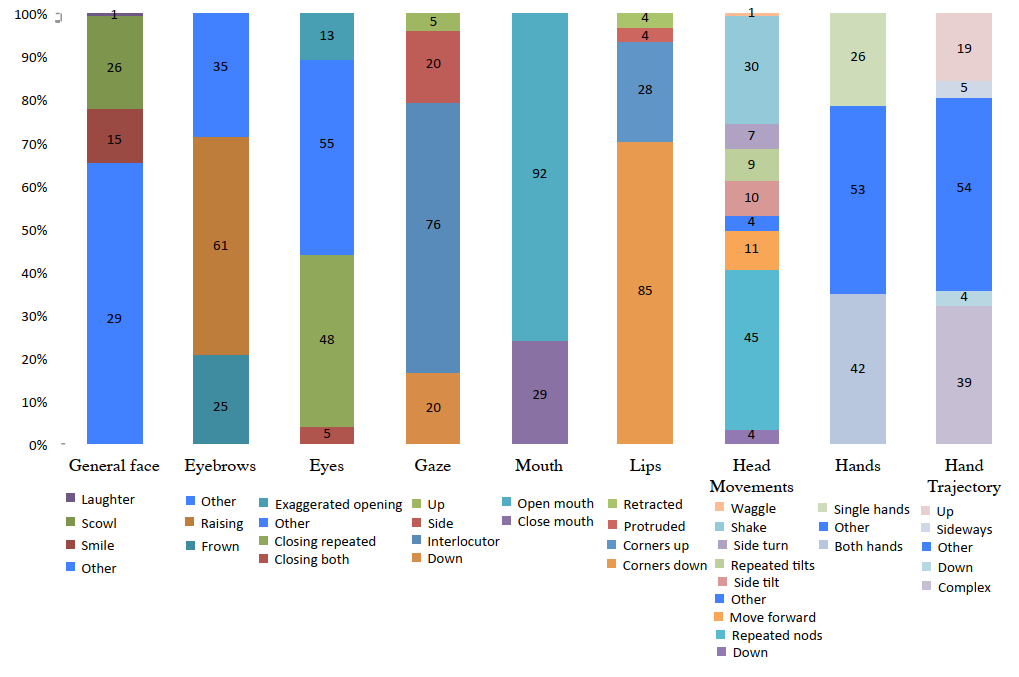
\includegraphics[width=1\textwidth]{rldb_distrib}
	\caption{Frequency of gestures annotated in the videos from the database. \cite{Perez-Rosas:2015:DDU:2818346.2820758}.}
	\label{fig:rldb_distrib}
\end{figure}

%TODO: rewrite tentative atm

We modified this database in the following way:
\begin{itemize}
	\item We cut or removed videos where the where the face was covered, hidden or in very difficult to see.
	\item We also cut parts of video that had multiple subjects in the scene because Action Unit extraction works on one person only.
	\item Since it is necessary to see the person to perform AU extraction, we also avoided some videos in which the subject was not visible while talking (the interlocutor was shown).
\end{itemize}

With deceptive videos going from \#1 to \#61 and truthful videos going from \#1 to \#60 we cut and removed the following videos from the original dataset, since they showed signs of the problems just described:

\begin{itemize}
	\item \textbf{Deceptive}:
	\begin{itemize}
		\item CUT: Video numbers 46, 47, 48, 49, 52, 54, 56.
		\item REMOVED: Video numbers 50, 53,  55.
	\end{itemize}
	\item \textbf{Truthful}:
	\begin{itemize}
		\item CUT: Video number 7, 28, 43.
		\item REMOVED: Video numbers 12, 31. 
	\end{itemize}
\end{itemize}


We also performed a division of subjects in the training and test set "by hand", splitting data to around 75\% for the training set and 25\% for the test set, to train the classifiers in a way that it wouldn't adapt the specific people since there are many videos with the same subject. In fact, the same person never appears both in the training and in the test set.

The training set consists of 72451 observations of 36 variables, and the test set is 14198 observations.
%todo: stats of db, #of frames ecc

\clearpage

\section{Data Analysis} \label{data_an}
In the following sections we describe the methods used to analyze the data and the machine learning techniques to classify them. \\
We start with comparing the occurrences for deceptive and truthful videos on the training set (par. \ref{data_comp}), then look at the correlation between variables (par. \ref{corr}), then we explain how we used GLM (par. \ref{GLM}), Random Forest (par. \ref{rf}) and Support Vector Machines (par. \ref{SVM})

\subsection{Data Comparison} \label{data_comp}
The first thing I did, after cleaning the data, was to compare the extracted deceptive (Fig \ref{fig:au_occ_dec}) and truthful (Fig. \ref{fig:au_occ_truth}) AUs occurrences (only for presence, not intensity) from the training set, which is shown in Fig. \ref{fig:au_occ_comp}.

\begin{figure}[H]
	\centering
	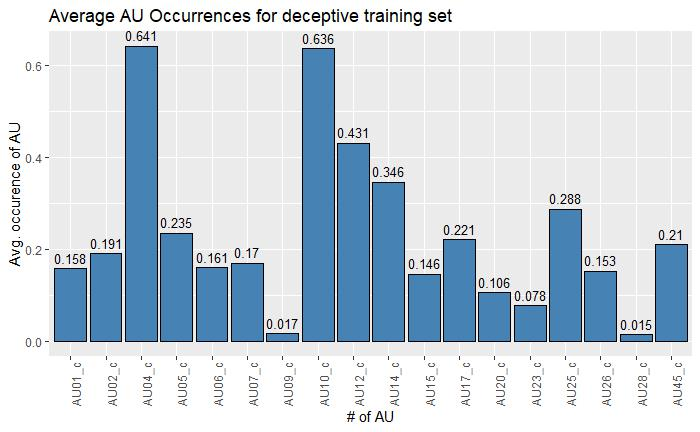
\includegraphics[width=1\textwidth]{images/au_occ_dec}
	\caption{Average AU Occurrences for the deceptive training set.}
	\label{fig:au_occ_dec}
\end{figure}

\clearpage

\begin{figure}[H]
	\centering
	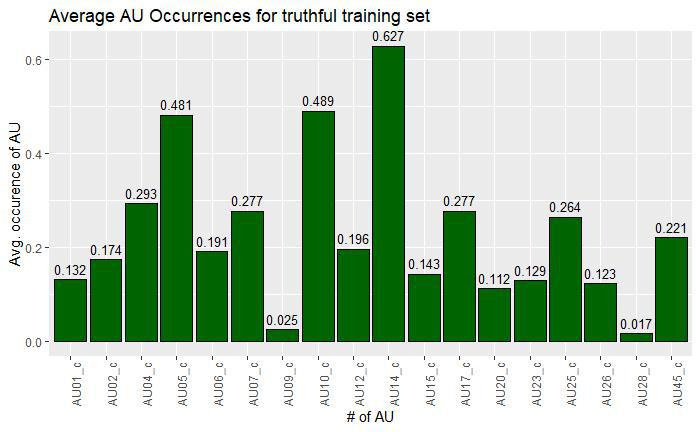
\includegraphics[width=1\textwidth]{images/au_occ_truth}
	\caption{Average AU Occurrences for the truthful training set.}
	\label{fig:au_occ_truth}
\end{figure}

\begin{figure}[H]
	\centering
	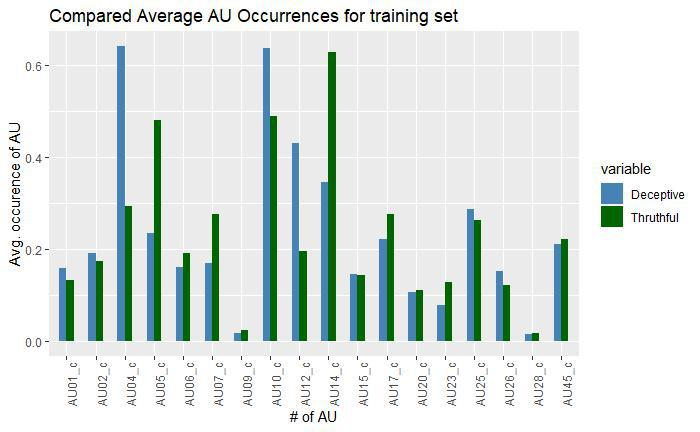
\includegraphics[width=1\textwidth]{images/au_occ_comp}
	\caption{Comparison of AU Occurrences for the training set.}
	\label{fig:au_occ_comp}
\end{figure}

This comparison shows interesting differences between truthful and deceptive occurrences for AU04 (Brow Lowerer), AU05 (Upper Lid Raiser), AU10 (Upper Lip Raiser), AU12 (Lip Corner Puller) and AU14 (Dimpler). %"suggesting there could be a pattern"?

\subsection{Correlation} \label{corr}
Variables correlation is shown in figure \ref{fig:correlation_matrix}. When the AUs label ends with "\_r" it indicate intensity and "\_c" means presence.

\begin{figure}[H]
	\centering
	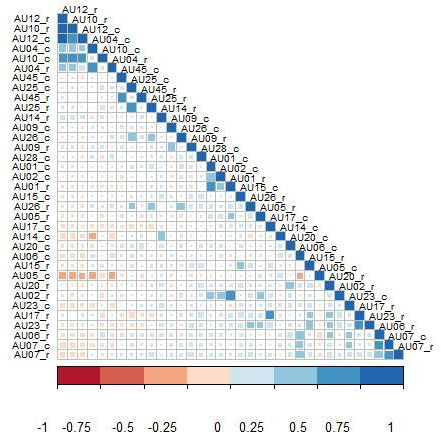
\includegraphics[width=1\textwidth]{images/correlation_matrix}
	\caption{Correlation between variables for both presence and intensity in the training set.}
	\label{fig:correlation_matrix}
\end{figure}

%todo: positive corr with, neg corr with... non tutte sono strong corr, forse cambiare un po'
which shows some obvious correlations between presence and intensity of the same AU, and significant correlation between AU10\_r, AU12\_r, AU12\_c, AU07\_r, AU17\_r, AU06\_r, AU04\_c, AU02\_r, AU01\_r, AU25\_r, AU45\_c.

\clearpage

\subsection{GLM} \label{GLM}
Another quick experiment I made was with the Generalized Linear Model in R, which translates into Logistic Regression (Par. \ref{logreg}), at least to have an idea of the resulting p-values, as seen in fig. \ref{fig:pval}:

\begin{figure}[H]
	\centering
	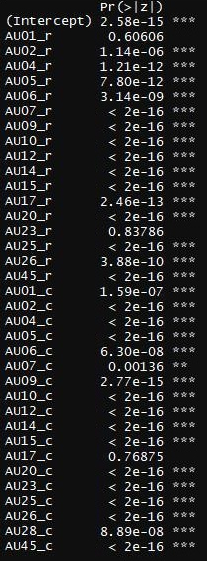
\includegraphics[width=0.4\textwidth]{images/pval}
	\caption{p-values from GLM for each AU (intensity and presence).}
	\label{fig:pval}
\end{figure}

As we can see AU01\_r (Inner Brow Raiser), AU23\_r (Lip Tightener), and AU17\_c (Chin Raiser) are not significant and that's an indication that we could remove them from the features used to make the classification.

%todo: should i say this?
The results for classifying data with GLM is 54.86\% accuracy on the test set, which is a little better than chance but not great. 

\clearpage

\subsection{Random Forest} \label{rf}
I've decided to use Random Forest (par. \ref{random_forest}) to estimate variable importance, shown in fig. \ref{fig:varimp}.

\begin{figure}[H]
	\centering
	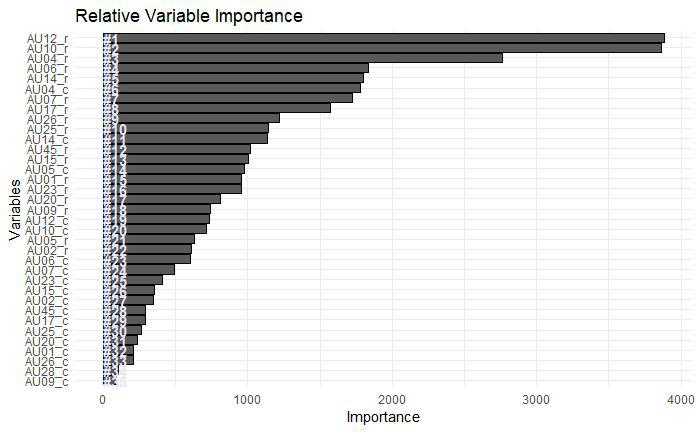
\includegraphics[width=1\textwidth]{images/varimp}
	\caption{Variable Importance extracted from classifying data with Random Forest.}
	\label{fig:varimp}
\end{figure}

The number of grown trees are 200 as going further did not increase the prediction accuracy at all.

Fig. \ref{fig:varimp} shows that the intensity of AUs 04, 06, 07, 10, 12 and 14 are the most significant, while the sole presence of an AU is not particularly significant, beside for AUs 04, 05 and 14.

As we can see AUs that have low p-values in GLM have also low importance in Random Forest.

Classifying with Random Forest gave me 58,42\% accuracy on the test set, which is better than GLM but it is still not good enough to be significant.

\clearpage

\subsection{SVM} \label{SVM}
%todo: some kind of image?
To approach classification with an SVM we tried both linear, radial and sigmoid kernel.

The cost $c$ and $\gamma$ parameter were found using a tuning function that performs a grid search over the combinations of cost and gamma for all the kinds of kernels we used, and then by empirically changing the values to see if better results could be achieved. 

In the tuning function $\gamma$ varied from $10^{-5}$ to $10^{-1}$ and \textit{c} from $10^{-3}$ to $10^2$. 

After the grid search I did some experimental changes and found empirically that the best parameters for the linear kernel were $C = 1$ and $\gamma = 0.04$

The results for classifying with a linear kernel are 67\% accuracy on the test set (to be precise 66.99394), which is a good starting result, while the radial kernel performed worse at around 61\% accuracy.

The best scoring kernel was actually the sigmoid kernel, giving us 68,64206\% accuracy when predicting the test set, by setting $\gamma  = 0.001$ and $C = 3$, obtaining the values of the parameters via both the tuning function and trial and error.

\clearpage

%todo: complete?
\section{Results} \label{results}
Using Support Vector Machine we were able to classify deceptive and truthful videos with an accuracy of 68,64\%.

The table below shows a comparison of the results obtained using different machine learning algorithms, and different kernels for SVM.

\begin{table}[H]
	\centering
	\begin{tabular}{|l|l|}
		\hline
		\textbf{Algorithm}  & \textbf{Accuracy} \\ \hline
		Logistic Regression & 54.86             \\ \hline
		Random Forest       & 58,42             \\ \hline
		SVM - Radial        & 61,56             \\ \hline
		SVM - Linear        & 66,99             \\ \hline
		SVM - Sigmoid       & 68,64             \\ \hline
	\end{tabular}
	\caption{Comparison of the results obtained with different approaches for this dataset}
\end{table}